Transfer learning is a machine learning technique in which the knowledge gained from one domain is transferred to a different but related problem. Recently, transfer learning has gained in popularity in computer vision problems after the success of~\cite{donahue2014decaf},~\cite{razavian2014cnn}, and~\cite{sermanet2013overfeat}. Yosinski et al.~\cite{yosinski2014transferable} defines a way to assess the transferability of features from different layers in deep neural networks and shows two cases where the performance drops after feature transferring, (1) when transferring features that are highly specialized in the first task, and (2) from optimization difficulties due to the splitting of the original network that leads to fragile co-adaption between units in consecutive layers. Azizpour et. al~\cite{azizpour2016factors} identified several factors that affects the transferability of features. Also they give advice on how to maximize the performance of a generic CNN when applied to a new task based on the similarity between the two tasks.

As discussed earlier in the case of image classification, CNNs extract features later used by the fully connected layers to classify the image (Figure~\ref{fig:transfer_learning}). Multiple CNNs (VGG16, VGG19, ResNet50, InceptionV3, etc.)  are available that are trained on large datasets such as ImageNet. These architectures have been trained on millions of images and classify the images to one of 1000 categories, such as car, airplane, etc. So transfer learning can be used in two ways:

\begin{itemize}
  \item The output of a layer can be used as features that are fed as input to a separate classifier (Figure~\ref{fig:VGG16_transfer_learning_feature_extractor}).
  \item Fine-tuning the entire network if the new dataset is similar to the original dataset, or freezing the first few layers as these layers detect edges and blobs and fine-tune the rest of the network (Figure~\ref{fig:VGG16_transfer_learning_finetuning}).
\end{itemize} 

\begin{figure}[]
    \begin{center}
    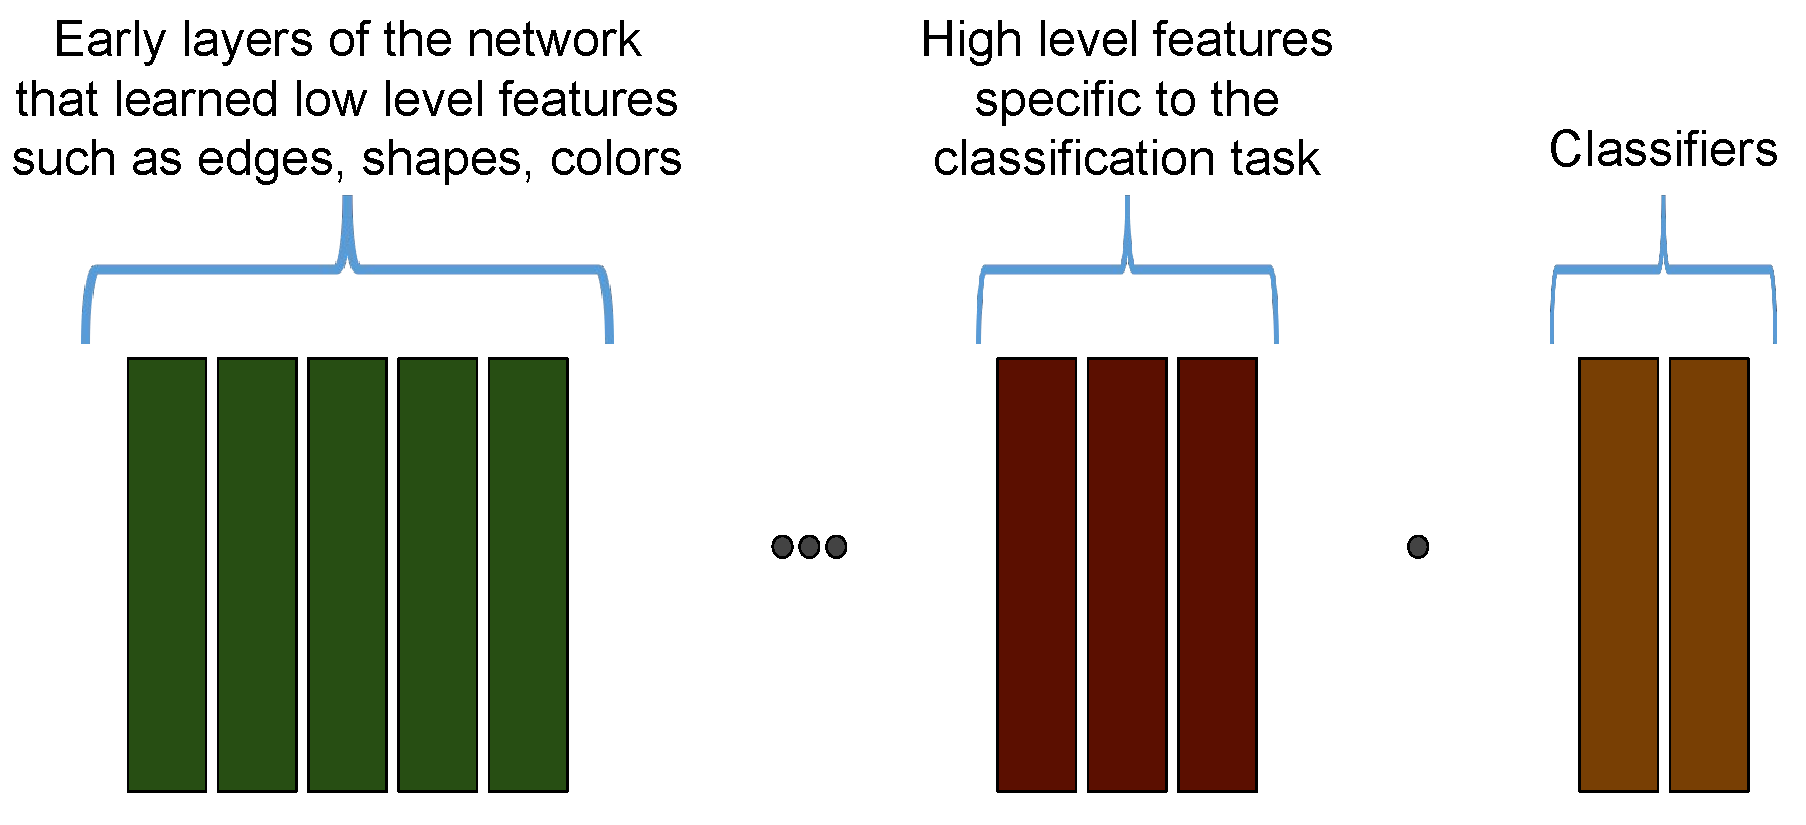
\includegraphics[width=0.8\textwidth]{images/transfer_learning.pdf}
    \end{center}
    \caption{Feature extraction from Convolutional Neural Network.} \label{fig:transfer_learning}
\end{figure}

\begin{figure}[]
    \begin{center}
    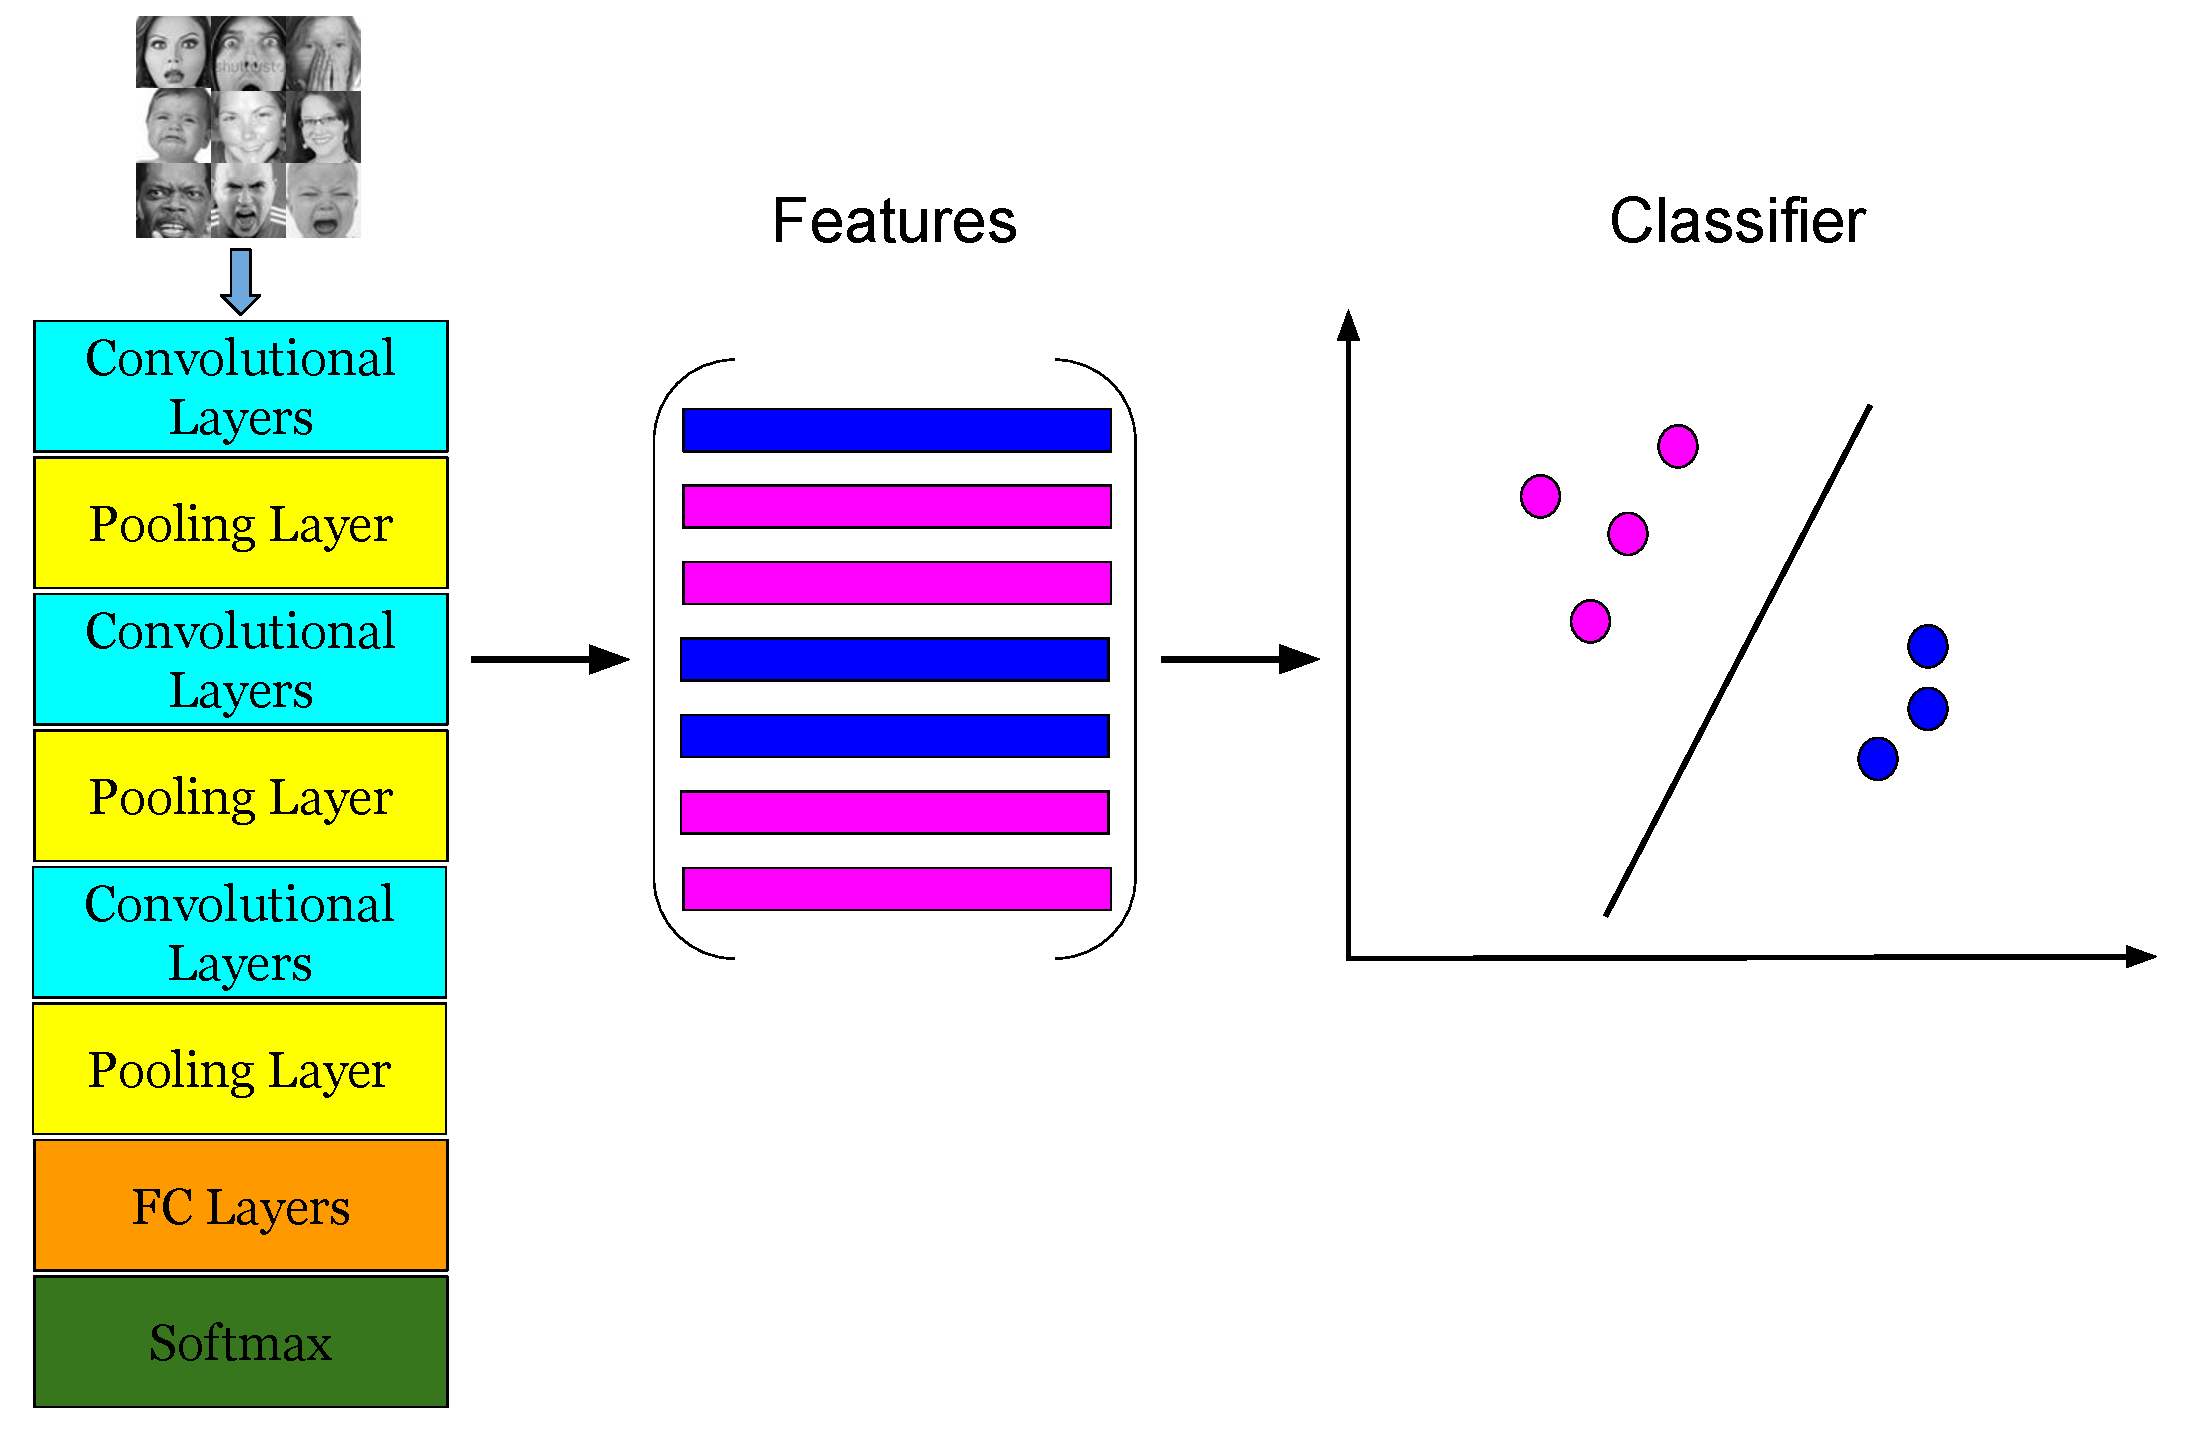
\includegraphics[width=0.8\textwidth]{images/VGG16_transfer_learning_feature_extractor.pdf}
    \end{center}
    \caption{Feature extraction from a pre-trained Convolutional Neural Network.} \label{fig:VGG16_transfer_learning_feature_extractor}
\end{figure}

\begin{figure}[]
    \begin{center}
    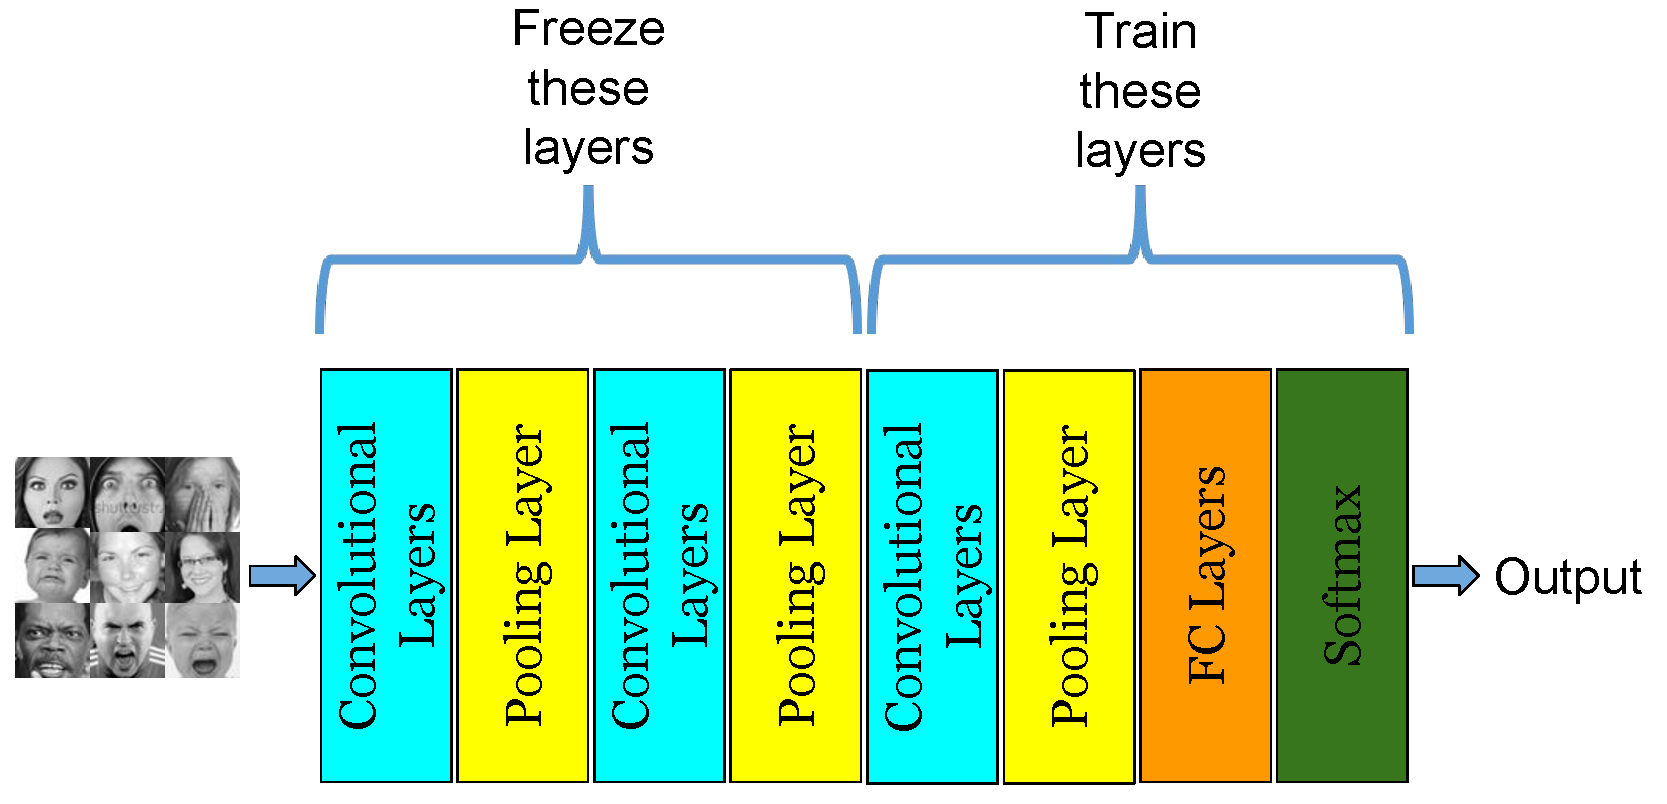
\includegraphics[width=0.8\textwidth]{images/VGG16_transfer_learning_finetuning.pdf}
    \end{center}
    \caption{Fine-tuning the pre-trained network.} \label{fig:VGG16_transfer_learning_finetuning}
\end{figure}


% \afterpage{\blankpage}